\documentclass[sigconf,authordraft]{acmart}

%%
%% \BibTeX command to typeset BibTeX logo in the docs
\AtBeginDocument{%
  \providecommand\BibTeX{{%
    \normalfont B\kern-0.5em{\scshape i\kern-0.25em b}\kern-0.8em\TeX}}}

%% Rights management information.  This information is sent to you
%% when you complete the rights form.  These commands have SAMPLE
%% values in them; it is your responsibility as an author to replace
%% the commands and values with those provided to you when you
%% complete the rights form.
\setcopyright{acmcopyright}
\copyrightyear{2020}
\acmYear{2020}
%\acmDOI{10.1145/1122445.1122456}

%% These commands are for a PROCEEDINGS abstract or paper.
\acmConference[PEARC '20]{PEARC '20}{July 26-30, 2020}{Portland, OR }
%\acmBooktitle{Woodstock '18: ACM Symposium on Neural Gaze Detection,
%  June 03--05, 2018, Woodstock, NY}
%\acmPrice{15.00}
%\acmISBN{978-1-4503-XXXX-X/18/06}


%%
%% Submission ID.
%% Use this when submitting an article to a sponsored event. You'll
%% receive a unique submission ID from the organizers
%% of the event, and this ID should be used as the parameter to this command.
%%\acmSubmissionID{123-A56-BU3}

%%
%% The majority of ACM publications use numbered citations and
%% references.  The command \citestyle{authoryear} switches to the
%% "author year" style.
%%
%% If you are preparing content for an event
%% sponsored by ACM SIGGRAPH, you must use the "author year" style of
%% citations and references.
%% Uncommenting
%% the next command will enable that style.
%%\citestyle{acmauthoryear}

%%
%% end of the preamble, start of the body of the document source.
\begin{document}

%%
%% The "title" command has an optional parameter,
%% allowing the author to define a "short title" to be used in page headers.
\title{Benchmark informed software upgrades at Quest-NUiT}

%%
%% The "author" command and its associated commands are used to define
%% the authors and their affiliations.
%% Of note is the shared affiliation of the first two authors, and the
%% "authornote" and "authornotemark" commands
%% used to denote shared contribution to the research.
\author{Sajid Ali}
\orcid{0000-0003-2186-4636}
\affiliation{%
  \institution{Applied Physics, Northwestern University}
  \streetaddress{2145 Sheridan Road}
  \city{Evanston}
  \state{Illinois}
  \postcode{60208}
}
\email{sajidsyed2021@u.northwestern.edu}

\author{Alper Kinaci}
\affiliation{%
\institution{NUiT RCS, Northwestern University}
  \streetaddress{2145 Sheridan Road}
  \city{Evanston}
  \state{Illinois}
  \postcode{60208}
  }
\email{akinaci@northwestern.edu}

%%
%% By default, the full list of authors will be used in the page
%% headers. Often, this list is too long, and will overlap
%% other information printed in the page headers. This command allows
%% the author to define a more concise list
%% of authors' names for this purpose.
%%\renewcommand{\shortauthors}{Trovato and Tobin, et al.}

%%
%% The abstract is a short summary of the work to be presented in the
%% article.
\begin{abstract}
  We present the work performed at Quest, a high performance computing cluster at Northwestern University regarding benchmarking of software perfromed to guide software upgrades. We performed extensive evaluation of all mpi libraries present on the system for functionality and performance in addition to testing architecture optimized software that can be loaded dynamically at runtime.
\end{abstract}

%%
%% The code below is generated by the tool at http://dl.acm.org/ccs.cfm.
%% Please copy and paste the code instead of the example below.
%%
\begin{CCSXML}
	<ccs2012>
	<concept>
	<concept_id>10011007.10011006.10011071</concept_id>
	<concept_desc>Software and its engineering~Software configuration management and version control systems</concept_desc>
	<concept_significance>500</concept_significance>
	</concept>
	<concept>
	<concept_id>10011007.10011006.10011073</concept_id>
	<concept_desc>Software and its engineering~Software maintenance tools</concept_desc>
	<concept_significance>300</concept_significance>
	</concept>
	</ccs2012>
\end{CCSXML}

\ccsdesc[500]{Software and its engineering~Software configuration management and version control systems}
\ccsdesc[300]{Software and its engineering~Software maintenance tools}

%%
%% Keywords. The author(s) should pick words that accurately describe
%% the work being presented. Separate the keywords with commas.
\keywords{software management, 	software builds, software automation}

%%
%% This command processes the author and affiliation and title
%% information and builds the first part of the formatted document.
\maketitle

\section{Introduction}
Software stack management is complex. We want to improve it.


\section{MPI}
Our benchmarks.


\subsection{Improvements}

\subsubsection{UCX}
\subsubsection{PMIx}

\section{Node arch dependent software}
\subsection{benchmarks}
\subsubsection{LAMMPS}
\subsubsection{GROMACS}



\section{Figures}

The ``\verb|figure|'' environment should be used for figures. One or
more images can be placed within a figure. If your figure contains
third-party material, you must clearly identify it as such, as shown
in the example below.
\begin{figure}[h]
  \centering
  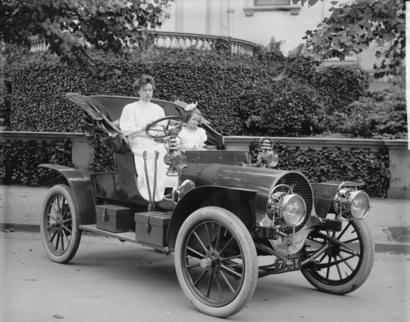
\includegraphics[width=\linewidth]{sample-franklin}
  \caption{A figure}
  \Description{The 1907 Franklin Model D roadster.}
\end{figure}

Your figures should contain a caption which describes the figure to
the reader. Figure captions go below the figure. Your figures should
{\bfseries also} include a description suitable for screen readers, to
assist the visually-challenged to better understand your work.

Figure captions are placed {\itshape below} the figure.




%%
%% The acknowledgments section is defined using the "acks" environment
%% (and NOT an unnumbered section). This ensures the proper
%% identification of the section in the article metadata, and the
%% consistent spelling of the heading.
\begin{acks}
To Alex from NUiT for help, to various mailing lists and forums including but not limited to mpich-discuss, slurm-info, spack-users.
\end{acks}

%%
%% The next two lines define the bibliography style to be used, and
%% the bibliography file.
\bibliographystyle{ACM-Reference-Format}
\bibliography{sample-base}

%%
%% If your work has an appendix, this is the place to put it.
%\appendix
%\section{Research Methods}
%\subsection{Part One}
%Lorem ipsum dolor sit amet, consectetur adipiscing elit. Morbi
%\subsection{Part Two}
%Etiam commodo feugiat nisl pulvinar pellentesque. Etiam auctor sodales
%\section{Online Resources}
%Nam id fermentum dui. Suspendisse sagittis tortor a nulla mollis, in

\end{document}
\endinput
%%
%% End of file `sample-authordraft.tex'.
